\documentclass[11pt]{article}
\usepackage[preprint]{neurips_2025}
\usepackage[utf8]{inputenc}
\usepackage[T1]{fontenc}
\usepackage{hyperref}
\usepackage{url}
\usepackage{booktabs}
\usepackage{amsfonts}
\usepackage{amsmath}
\usepackage{amssymb}
\usepackage{nicefrac}
\usepackage{microtype}
\usepackage{graphicx}
\usepackage{multirow}
\usepackage{makecell}
\usepackage{enumitem}
\usepackage[normalem]{ulem}  % \uline for line-breakable underline; normalem preserves \emph italics


\title{Mitigating Shortcut Reasoning in Language Models: A Gradient-Aware Training Approach}


\author{
Hongyu Cao \\
Arizona State University \\
\texttt{hongyuca@asu.edu}
\And
Kunpeng Liu \\
Clemson University \\
\texttt{kunpenl@clemson.edu}
\And
Dongjie Wang \\
University of Kansas \\
\texttt{wangdongjie100@gmail.com}
\And
Yanjie Fu \\
Arizona State University \\
\texttt{yanjiefu@asu.edu}
}

\begin{document}
\maketitle
\iffalse
\begin{abstract}
Reasoning failures in language models often arise not because training data are mislabeled, but because some examples reduce loss through shortcut updates---surface patterns, answer templates, or spurious correlations that do not support generalization. We study where this distinction appears during training and show that shortcut behavior is more directly revealed by \emph{gradient geometry} than by scalar loss: shortcut-promoting samples exhibit two observable signatures, low alignment with a small validation gradient that reflects generalizable reasoning, and concentrated gradient energy on answer tokens rather than on intermediate reasoning tokens. This yields a directional view of shortcut-aware reasoning training. The goal is not to decide which samples to keep, but which components of each sample's gradient to trust. We instantiate the view in \textbf{SART}, a detection-then-correction framework that ranks samples by a \textsc{ShortcutScore} and applies a per-sample, conflict-only projection that removes only the component opposing the validation gradient. Across three controlled reasoning benchmarks, SART improves over the strongest of eleven baselines by $+4.7$\,pp accuracy and $+7.1$\,pp robustness, with the conflict-gated projection alone contributing $+36.5$\,pp robustness in ablations shows that directional correction, not detection accuracy, is the load-bearing mechanism. A Qwen3-8B / GSM8K pilot shows the detection geometry transfers cleanly to pretrained LLMs, while correction at this scale must respect autoregressive generation constraints, which is a constrained variant of the same principle. Overall, this paper proves the principle and mechanism under controlled shortcut injection, shows that detection transfers to LLM scale, and leaves full LLM correction as a constrained scaling problem---reframing shortcut mitigation as a problem of gradient alignment and directional correction, rather than only loss shaping or sample filtering.
\end{abstract}
\fi

\begin{abstract}
Reasoning failures in language models often arise not because training data are mislabeled, but because some examples reduce loss through shortcut updates: surface patterns, answer templates, or spurious correlations that do not support generalization. We show that this failure is structurally hidden along three axes: (i) loss ambiguity, where shortcut and reasoning samples can have similar scalar losses; (ii) sample ambiguity, where one example contains both useful reasoning signal and harmful shortcut signal; and (iii) correction ambiguity, where filtering or reweighting changes which samples are used or how strongly, but not which gradient directions are trusted. We argue that reliable shortcut mitigation requires operating on gradient-level alignment rather than scalar loss or sample identity.
We propose Shortcut-Aware Reasoning Training (SART), a detection-then-correction framework with two components. First, \textsc{ShortcutScore} ranks samples by low alignment with a small validation gradient and high concentration of gradient energy on final-answer tokens. Second, SART applies a per-sample, conflict-only projection that removes only the component of a flagged gradient opposing the validation gradient, while preserving its aligned residual. Across three controlled reasoning benchmarks, SART improves over the strongest of eleven baselines by $+4.7$ pp accuracy and $+7.1$ pp robustness. Ablations show that directional correction is the load-bearing mechanism: removing conflict-only projection reduces robustness by $36.5$ pp, while scalar reweighting achieves higher detection F1 but worse generalization. A Qwen3-8B/GSM8K pilot shows that detection transfers to pretrained LLMs, while full correction must respect autoregressive generation constraints. These results suggest that shortcut mitigation does not lack useful training signal; it lacks directional discrimination.
\end{abstract}

\section{Introduction}

Large language models (LLMs) deployed in high-stakes reasoning tasks frequently exploit \textit{reasoning shortcuts}—surface pattern matching, answer memorization, keyword-answer correlations, and premature answer prediction—rather than performing genuine logical inference~\cite{wei2022chain,wang2022self}. This shortcut reliance stems from \textbf{training signal misalignment}: shortcut-encouraging samples efficiently reduce training loss but fail to foster generalizable reasoning. Consequently, models accurate on training distributions fail catastrophically when numbers change, constraints vary, or problem phrasing shifts. This motivates \textit{\textbf{S}hortcut-\textbf{A}ware \textbf{R}easoning \textbf{T}raining (SART)}: identifying samples that promote shortcut updates and modifying gradient dynamics to emphasize genuine reasoning signals. Solving SART is critical for reliable LLM deployment in mathematical reasoning, financial analysis, planning, and scientific discovery—domains where spurious reasoning leads to incorrect decisions or unsafe recommendations.


Two major challenges arise in solving SART: (1) detecting shortcut-promoting samples from gradient behavior, and (2) modifying training dynamics to suppress shortcut learning without degrading performance. First, shortcut samples are often correctly labeled and indistinguishable by conventional quality metrics. They produce strong gradients that efficiently reduce training loss, making loss-based detection unreliable. The detection challenge is: how can we identify training samples whose gradients improve loss but harm reasoning generalization? Second, simply down-weighting or removing detected shortcut samples is insufficient—it destabilizes training and discards useful signal. The suppression challenge is: how can we modify training dynamics to neutralize shortcut gradients while preserving generalizable reasoning signals from the same samples?

Existing methods only partially address SART. Chain-of-Thought (CoT) training~\cite{wei2022chain,kojima2022large} encourages intermediate reasoning traces but does not modify training dynamics: models can generate plausible steps that still rely on shortcuts, and shortcut gradients remain dominant~\cite{ho2022large}. Self-Consistency Decoding~\cite{wang2022self} samples multiple reasoning paths to detect inconsistencies but operates at inference time, leaving shortcut patterns intact in model parameters. Data filtering and curriculum learning~\cite{bengio2009curriculum} attempt to remove noisy samples, but shortcut samples are typically correctly labeled, making them invisible to label-quality filters. RLHF~\cite{ouyang2022training} optimizes reward signals based on answer correctness rather than reasoning validity, allowing shortcuts to persist when they produce correct answers. These approaches cannot jointly address shortcut detection from gradient behavior and dynamic suppression during training—a gradient-centric perspective is required.

\textbf{Our insights: gradient-aware shortcut detection and correction.} We formulate SART as a gradient structure analysis problem. We find that shortcut reasoning samples produce two distinct gradient signatures: (1) \textit{low alignment} with gradients that improve held-out validation performance, indicating the sample's gradient direction does not transfer to generalizable reasoning; and (2) \textit{high answer-token concentration}, where gradient norms are dominated by final answer tokens rather than intermediate reasoning tokens. These signals—gradient alignment with validation gradients and answer-gradient concentration—can be combined into a principled \textbf{ShortcutScore} quantifying the degree to which a sample promotes shortcut learning. Furthermore, harmful shortcut gradient directions can be neutralized via \textit{gradient surgery}: projecting gradients orthogonally onto subspaces that avoid non-transferable directions, forcing the model to learn from genuine reasoning signals without discarding samples entirely.

\textbf{Proposed Approach.} This paper presents the first principled shortcut-aware training framework for LLM reasoning via gradient structure analysis, with two goals: (1) precise detection of shortcut-promoting samples through gradient behavior; (2) effective suppression of shortcut learning while preserving generalizable reasoning signals.
%
For Goal 1, we develop the \textbf{ShortcutScore}, a composite metric combining cosine similarity between per-sample gradients and validation gradients (measuring non-transfer alignment) with the ratio of answer-token to reasoning-token gradient norms (measuring answer-dominant credit assignment). Samples with high ShortcutScore are flagged as shortcut-promoting.
%
For Goal 2, we develop a \textbf{gradient surgery} technique that identifies harmful gradient directions—those misaligned with validation gradients or increasing ShortcutScore—and projects them orthogonally to suppress their influence during parameter updates. This ensures training dynamics prioritize reasoning token signals.

Our framework is model-agnostic and integrates into any LLM training pipeline without architectural changes. Extensive experiments across mathematical reasoning, commonsense reasoning, and constraint-based planning benchmarks demonstrate significant improvements in robustness under distribution shift, number perturbation, and phrasing variation, validating that our approach reduces shortcut reliance and promotes genuine logical inference. Code is available at \url{https://github.com/fuyanjie/short-cut-aware-data-centric-reasoning}.
\section{Problem Statement}

\textbf{The SART Problem.}
We study supervised training of language models on reasoning tasks. Let $\mathcal{D} = \{(x_i, y_i)\}_{i=1}^{N}$ be a training dataset where $x_i$ is an input reasoning problem and $y_i$ is the corresponding output comprising intermediate reasoning steps and a final answer. Let $\mathcal{V} = \{(x_j, y_j)\}_{j=1}^{M}$ be a small held-out validation set drawn from a distribution that rewards genuine reasoning, and let $\theta$ denote the parameters of a language model $f_\theta$. Standard training minimizes the empirical risk:
\begin{equation}
    \min_{\theta} \; \frac{1}{N} \sum_{i=1}^{N} \ell(\theta;\, x_i, y_i),
\end{equation}
where $\ell$ is the token-level negative log-likelihood loss. This objective does not distinguish between samples that promote genuine logical inference and those that achieve low loss via superficial patterns---keyword-answer correlations, answer token memorization, or template matching. We call such samples \emph{shortcut reasoning samples}.

Formally, let $\mathbf{g}_s = \nabla_\theta\, \ell(\theta; s)$ denote the gradient of a training sample $s = (x, y)$, and let
\begin{equation}
    \mathbf{g}_{\mathcal{V}} = \nabla_\theta \; \frac{1}{|\mathcal{V}|} \sum_{v \in \mathcal{V}} \ell(\theta;\, v)
\end{equation}
be the validation gradient, reflecting parameter updates that improve generalizable reasoning. A sample $s$ is a shortcut reasoning sample if $\mathbf{g}_s$ (i) exhibits low alignment with $\mathbf{g}_{\mathcal{V}}$, indicating the update does not transfer to genuine reasoning, and (ii) concentrates gradient norm on final answer tokens rather than intermediate reasoning tokens, indicating the model learns \emph{what to answer} rather than \emph{how to reason}. Critically, such samples are often correctly labeled and efficiently reduce training loss, rendering them undetectable by conventional data quality, label-noise, or scalar-loss metrics.

\textbf{Shortcut-Aware Reasoning Training (SART)} formulates the problem as a two-step gradient-geometry detection-then-correction task. Concretely, we pursue two objectives: 1) \textbf{detection}: rank training samples by gradient-derived shortcut tendency, given by a \textsc{ShortcutScore} $S(s)$ that combines non-transfer alignment with answer-token concentration; 2) \textbf{conditional correction}: for samples flagged as shortcut-prone, project out only the component of $\mathbf{g}_s$ that genuinely opposes $\mathbf{g}_{\mathcal{V}}$, leaving validation-aligned directions intact. Formally, with $\mathcal{S}^\star = \{s : S(s) > \tau_S^\star\}$ the flagged set and $\mathbf{g}_s'$ the corrected per-sample gradient, SART solves
\begin{equation}
    \min_{\theta} \; \frac{1}{N}\sum_{i=1}^{N} \ell(\theta;\, x_i, y_i)
    \quad \text{subject to} \quad
    \mathbf{g}_s'^{\top} \mathbf{g}_{\mathcal{V}} \;\geq\; 0 \;\;\text{for all } s \in \mathcal{S}^\star,
\end{equation}
where the constraint is realized by a conflict-only PCGrad-style projection on the per-sample gradient before batch aggregation; samples with $s \notin \mathcal{S}^\star$ contribute their original gradient at unit weight. The framework operates purely at the level of training dynamics, requiring neither architectural modifications nor shortcut-group / multi-environment annotations.

\section{Overview}

% =============================================================================
% PAPER-LEVEL TODO INDEX  (last updated 2026-04-25, commit after 1a44f69)
%
% Each item has a more detailed --TODO-- block at the relevant LaTeX site;
% this index is the quick map. Cross-refs:
%   docs/experiments/shortcut_score_followups.qmd  (Gaps 1..6)
%   docs/experiments/hyperparam_followups.qmd      (Issues 1..3)
%   docs/experiments/pcgrad_rerun.qmd              (PCGrad / 12-baseline)
%   docs/experiments/llm_gsm8k.qmd                 (LLM transfer follow-ups)
%
% [DONE]   3_overview.tex figure replaced with TikZ method illustration
%          (figures/sart_method_figure.{tex,png}); original PNG preserved
%          (figures/short_cut_aware_framework.png is untouched).
%
% [OPEN]   §5.2 (sec:exp_detection) — paragraph-level rewrite.
%          Why open: Gap 4 sweep (commit 1c8e7c8) showed r=0.67 is reproducible
%          ONLY at Math K=3, never as 3-dataset aggregate; Gap 5 (commit
%          3e27cf9) showed Reweight-Only's +robustness gain is decoupled from
%          the score's r calibration. Current §5.2 prose treats r=0.67 as a
%          stable property and attributes the gain to score-driven correction;
%          both framings are empirically refuted.
%          Action: replace the bin-scatter at one cherry-picked state with the
%          per-dataset r-vs-K curves (results/warmup_sweep.png), and recast
%          the "F1=0.64 + soft action" account into a "weighted-retraining-
%          duration" account. This is pure prose work — no GPU needed.
%
% [OPEN]   §5.3 (sec:exp_sensitivity) — three hyperparameter follow-ups.
%          Issue 1: tau_A / tau_R / alpha / beta scale-mismatch.
%          Issue 2: rho=0.5 (main) vs rho=0.3 (appendix). Decision pending:
%                   Option A (single default) vs Option B (per-task tuning).
%          Issue 3: gamma depends on unobservable shortcut compositional
%                   complexity at deployment.
%          Issue 2 is the highest-priority one (internal inconsistency that
%          a referee will flag immediately).
%
% [OPEN]   §5 — reproduction gap on Reweight-Only's reported +20.7 pp
%          robustness vs our K=8 measurement (+8.1 pp). ~2.5x gap unexplained.
%          Possible causes: lambda tuning, score-pass timing, selection
%          effects in the original numbers.
%
% [OPEN]   Gap 6: full SART (Reweight + Surgery) K-sensitivity sweep.
%          ----- See longer note in 5_experiment.tex §5.2 TODO block. -----
%          A "K-sensitivity sweep" varies the warmup-K hyperparameter, runs
%          the full method end-to-end at each K, and measures the final
%          accuracy / robustness. The OUTPUT is a metric-vs-K curve. The
%          PURPOSE here is mechanism diagnosis — does full SART's accuracy
%          / robustness depend on the score's calibration at that K? — NOT
%          method selection (we already know the score's calibration is
%          dataset-specific; recommending one K as a deployment default is
%          ruled out by Gap 4). Three possible outcomes:
%            (a) Full SART is K-sensitive in the same way as Reweight-Only:
%                surgery is also score-independent. The whole "detection +
%                correction" framing needs deeper revision.
%            (b) Full SART is K-sensitive in a way that tracks the score's
%                r at each K: surgery is the load-bearing component, and
%                the score's calibration matters specifically for surgery
%                (not for reweight). Method retains its core claim.
%            (c) Full SART is K-INsensitive (flat curve): both components
%                decouple from score quality; the gain is purely from
%                training-time effects, and the paper's narrative around
%                S(s) needs broad revision.
%          Cost: ~50 min on a clean H100 NVL (mirrors reweight_only_K_sweep).
%          Script: copy scripts/reweight_only_K_sweep.py with
%          use_gradient_surgery=True.
%
% [OPEN]   12-baseline rerun under PCGrad-fixed (gamma=1.0, rho=0.3) defaults
%          (see pcgrad_rerun.qmd; currently SART-only is verified, full
%          baseline table is not).
%
% [OPEN]   LLM transfer follow-ups: numeric-only g_s_ans; hard-cut detection;
%          larger LoRA/epoch budget on Qwen3-8B GSM8K (llm_gsm8k.qmd).
%
% [HOLD]   Gap 3b — figure 2 structural restructure (merge w(s) into panel
%          (a) as twin axis; reuse panel (c) slot for FP-cell A(s) plot).
%          On hold pending Gap 6 outcome.
% =============================================================================

\begin{figure}
    \centering
    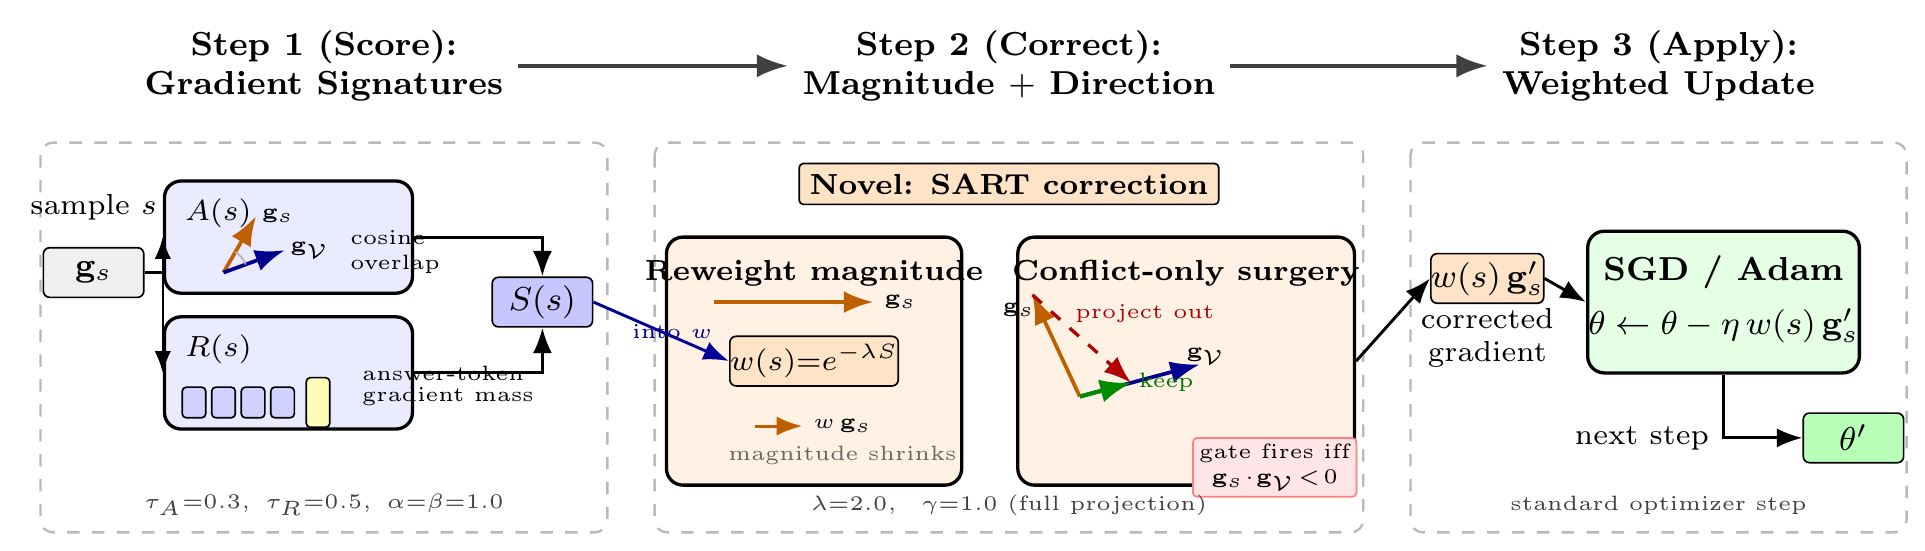
\includegraphics[width=\linewidth]{figures/sart_method_figure.png}
    \caption{
    Overview of SART. (A) Per-sample gradient alignment with validation gradients and answer-token concentration.
    (B) \textsc{ShortcutScore} combines both signals to flag shortcut-prone samples.
    (C) Exponential reweighting lowers their magnitude.
    (D) Conflict-only gradient surgery removes only the component that opposes $\mathbf{g}_{\mathcal{V}}$, preserving validation-aligned directions already present in $\mathbf{g}_s$.
    (E) Updates prioritize reasoning signals over shortcut patterns.
    }
    \label{fig:overview}
\end{figure}

Figure~\ref{fig:overview} illustrates the two coupled operations behind \textbf{shortcut-aware reasoning training (SART)}: \textsc{ShortcutScore}-based sample reweighting, and conflict-only gradient surgery. Detection reads two gradient signatures---\emph{non-transfer alignment} (low cosine with $\mathbf{g}_{\mathcal{V}}$, signalling updates that reduce loss without improving held-out reasoning) and \emph{answer-gradient concentration} (gradient energy dominated by final-answer tokens rather than intermediate reasoning tokens). Correction acts along two complementary axes: reweighting scales \emph{how much} each sample contributes, while conflict-gated surgery corrects \emph{in which direction} the update proceeds, projecting out only the component that genuinely opposes $\mathbf{g}_{\mathcal{V}}$ (PCGrad-style~\cite{yu2020gradient}) and leaving positively-aligned directions untouched. Section~\ref{sec:method} formalizes each step.

\section{Method}
\label{sec:method}

\subsection{ShortcutScore: Gradient-Structure Detection}

\noindent\textbf{Why Gradient-Structure Detection.}
Standard empirical risk minimization treats all training samples equally, optimizing the average token-level loss across the dataset. This is problematic because shortcut reasoning samples---those that achieve low loss by exploiting keyword correlations, answer memorization, or surface pattern matching---generate strong gradients that efficiently reduce training loss but do not support generalizable reasoning. Critically, such samples are often correctly labeled, making them invisible to conventional data quality filters or scalar loss-based criteria. We therefore detect shortcut-promoting samples from the geometry of their gradients rather than from labels or loss values, identifying two complementary geometric signatures: (1) \textbf{Non-Transfer Alignment.} per-sample gradients are poorly aligned with the validation gradient, signaling updates that reduce loss without improving held-out reasoning; (2) \textbf{Answer-Gradient Concentration.} gradient energy concentrates on final-answer tokens rather than intermediate reasoning tokens, signaling the model learns \emph{what to answer} rather than \emph{how to reason}. The detector is intentionally a \emph{rank} signal: it does not need to be a calibrated estimator of shortcut probability---only to order the samples well enough that the downstream surgery's per-sample conflict gate has the right working set to act on.

\noindent\textbf{Step 1: Non-Transfer Gradient Alignment.}
For each training sample $s = (x, y)$, we compute the per-sample gradient $\mathbf{g}_s = \nabla_\theta \ell(\theta; s)$ and the validation gradient
\begin{equation}
    \mathbf{g}_{\mathcal{V}} = \nabla_\theta \frac{1}{|\mathcal{V}|} \sum_{v \in \mathcal{V}} \ell(\theta; v).
\end{equation}
The non-transfer gradient alignment is then defined as:
\begin{equation}
    A(s) = \cos(\mathbf{g}_s,\, \mathbf{g}_{\mathcal{V}}) = \frac{\mathbf{g}_s^\top \mathbf{g}_{\mathcal{V}}}{\|\mathbf{g}_s\|\|\mathbf{g}_{\mathcal{V}}\|}.
\end{equation}
A low value of $A(s)$ indicates that the gradient of sample $s$ points in a direction inconsistent with improving validation reasoning performance---a hallmark of shortcut exploitation.

\noindent\textbf{Step 2: Answer-Gradient Concentration.}
Let $T_{\mathrm{ans}}$ and $T_{\mathrm{reason}}$ denote the index sets of answer tokens and reasoning tokens in the output sequence. The answer-gradient concentration is defined as
\begin{equation}
    R(s) = \frac{\sum_{t \in T_{\mathrm{ans}}} \|\nabla_\theta \ell_t\|}{\sum_{t \in T_{\mathrm{ans}} \cup T_{\mathrm{reason}}} \|\nabla_\theta \ell_t\|},
\end{equation}
where $\ell_t$ is the token-level loss at position $t$. A high value of $R(s)$ indicates that the model's parameter updates are driven predominantly by answer prediction rather than by learning intermediate reasoning steps. When a token-level answer/reasoning split is unavailable (answer-only supervision, $T_{\mathrm{reason}}{=}\emptyset$), we set $R(s){=}\tau_R$ so that $S(s)$ degenerates gracefully to an alignment-only score; Appendix~\ref{sec:appendix_graceful} gives the derivation.

\noindent\textbf{Step 3: ShortcutScore and Selection Set.}
The two signals combine into the \textbf{ShortcutScore}:
\begin{equation}
    S(s) = \alpha \cdot \max(0,\, \tau_A - A(s)) + \beta \cdot \max(0,\, R(s) - \tau_R),
\end{equation}
where $\tau_A$ and $\tau_R$ are thresholds defining low alignment and high concentration, and $\alpha, \beta$ are balancing hyperparameters (defaults in Appendix~\ref{sec:appendix_sensitivity}). Samples with high $S(s)$ are flagged as shortcut-promoting, forming the selection set
\begin{equation}
    \mathcal{S}^\star = \{\, s \in \mathcal{D} : S(s) > \tau_S^\star \,\},
\end{equation}
where $\tau_S^\star$ is set to the F1-optimal threshold on $S(s)$ over a held-out probe (in our experiments $\tau_S^\star \approx 0$, so the selection set is approximately the upper half of the score distribution; see \S\ref{sec:exp_detection}). Samples in $\mathcal{S}^\star$ enter the gradient-surgery step (\S\ref{sec:gradient_surgery}); samples outside $\mathcal{S}^\star$ contribute their gradient unchanged. The validation gradient $\mathbf{g}_{\mathcal{V}}$ is recomputed periodically to keep the alignment signal up to date without excessive overhead. Algorithmic details appear in Appendix~\ref{sec:appendix_algorithm}.


%-----------------------------------------------------------
\subsection{Conflict-Only Gradient Surgery}
\label{sec:gradient_surgery}

\noindent\textbf{Why Conflict-Only Surgery, Not Reweighting or Removal.}
Detection alone identifies which samples need intervention but does not modify a single update. Two natural correction strategies fail. (1) \textbf{Hard Removal.} Dropping the entire sample (e.g., data filtering or influence-based selection) discards the validation-aligned component the sample still carries. A shortcut-flagged sample is a \emph{mixed} object: even when its gradient direction is overall harmful, a non-trivial subspace of its gradient remains aligned with $\mathbf{g}_{\mathcal{V}}$, and that subspace would have helped training had it been preserved. (2) \textbf{Scalar Reweighting.} Multiplying the per-sample gradient by a continuous weight (e.g., $w(s) = \exp(-\lambda S(s))$) shrinks magnitude but leaves direction unchanged: a downweighted-but-still-pointing-the-wrong-way gradient is still pointing the wrong way. Empirically, scalar reweighting is decoupled from the detector's calibration and offers no gain over conflict-only surgery alone (see ablation in \S\ref{sec:exp_ablation}). The minimal correction that both (i) preserves the useful component of a shortcut sample and (ii) cancels its harmful direction is therefore \emph{conditional directional projection}: act on direction, not on magnitude, and act only when there is a genuine conflict to resolve. We instantiate this idea via a PCGrad-style~\cite{yu2020gradient} conflict-only projection, augmented with an optional answer-gradient suppression term where the second detection signal $R(s)$ indicates the gradient is dominated by answer tokens.

\noindent\textbf{Step 1: Conflict-Only Projection for Non-Transfer Alignment.}
For each $s \in \mathcal{S}^\star$, we remove the component of $\mathbf{g}_s$ that conflicts with $\mathbf{g}_{\mathcal{V}}$, following the PCGrad conflict-removal principle. Concretely, we project only when the two gradients genuinely disagree:
\begin{equation}
\label{eq:gradient_surgery}
    \mathbf{g}_s' =
    \begin{cases}
        \mathbf{g}_s - \gamma\,\dfrac{\mathbf{g}_s^\top \mathbf{g}_{\mathcal{V}}}{\|\mathbf{g}_{\mathcal{V}}\|^2}\,\mathbf{g}_{\mathcal{V}}, & \text{if } \mathbf{g}_s^\top \mathbf{g}_{\mathcal{V}} < 0, \\[4pt]
        \mathbf{g}_s, & \text{otherwise,}
    \end{cases}
\end{equation}
where $\gamma \in [0,1]$ is the projection strength ($\gamma{=}1$ fully removes the conflicting component). This conflict-gated rule is deliberately asymmetric: even a shortcut-flagged sample may carry a small positive alignment with $\mathbf{g}_{\mathcal{V}}$, and erasing that component would discard a validation-improving direction---the opposite of our goal. Projection fires only in the truly harmful case ($\mathbf{g}_s$ points \emph{against} validation), and the resulting $\mathbf{g}_s'$ then has non-negative inner product with $\mathbf{g}_{\mathcal{V}}$.

\noindent\textbf{Step 2: Suppression for Answer-Gradient Concentration.}
For $s \in \mathcal{S}^\star$ with $R(s) > \tau_R$, we further decompose $\mathbf{g}_s'$ into answer-token and reasoning-token components and suppress the answer-dominant part:
\begin{equation}
    \mathbf{g}_s'' = (1 - \rho)\,\mathbf{g}_s'^{\,\mathrm{ans}} + \mathbf{g}_s'^{\,\mathrm{reason}},
\end{equation}
where $\rho \in [0,1]$ is the suppression coefficient. Setting $\rho{=}0$ disables this term, recovering pure conflict-only projection; setting $\rho{=}1$ removes the answer-token gradient contribution entirely, forcing the model to update from intermediate reasoning signals only. Empirically, $\rho{>}0$ is beneficial on tasks whose shortcut signal manifests in answer tokens but harms autoregressive generation in large language models (see \S\ref{sec:exp_llm_transfer}); we therefore use $\rho{=}0$ as the default in the LLM regime.

\noindent\textbf{Combined Update Rule.}
At each training step, the per-sample gradient enters surgery only if $s \in \mathcal{S}^\star$. The batch gradient is the unweighted sum of corrected per-sample gradients, $\mathbf{g}_{\mathrm{batch}} = \sum_{s \in \mathrm{batch}, s \in \mathcal{S}^\star} \mathbf{g}_s'' \;+\; \sum_{s \in \mathrm{batch}, s \notin \mathcal{S}^\star} \mathbf{g}_s$, which then drives a standard optimizer step. The validation gradient $\mathbf{g}_{\mathcal{V}}$ is refreshed every $k$ steps (Section~\ref{sec:exp_llm_transfer}) so the conflict test and projection direction remain accurate. Pseudocode for the combined SART step is in Appendix~\ref{sec:appendix_algorithm}.

\paragraph{Scaling to pretrained LLMs.}
A naive implementation stores a dense per-sample gradient of dimension $|\theta|$, which is $\sim$28\,GB in FP32 for a 7B backbone. We keep SART tractable on pretrained LLMs by (i) restricting trainable capacity to LoRA adapters~\cite{hu2022lora} so each per-sample gradient collapses to $\sim$32\,MB without altering Eqs.~(5) or~(\ref{eq:gradient_surgery}); (ii) optionally replacing gradients by fixed-seed Johnson--Lindenstrauss sketches of dimension $d_{\mathrm{sk}}{=}1024$ during scoring, which preserves the cosine alignment $A(s)$ up to $\varepsilon$-error; and (iii) refreshing $\mathbf{g}_{\mathcal{V}}$ every $k$ steps rather than every step, since it changes slowly relative to $\theta$. These three mechanisms are orthogonal to the \textsc{ShortcutScore} and surgery formulations---any alternative inner-product-preserving proxy (Fisher-diagonal, last-layer gradients, influence approximations~\cite{koh2020understandingblackboxpredictionsinfluence}) can be slotted in without changing the method. Full derivations and ablations appear in Appendix~\ref{sec:scalable_gradients}.

\section{Experiments}
\label{sec:experiments}

We evaluate SART from a mechanism-first perspective. Rather than focusing only on end accuracy, we ask four questions: \textbf{(Q1)} can SART improve robustness under controlled shortcut settings where the ground-truth reasoning rule is known; \textbf{(Q2)} is directional correction---rather than detection accuracy alone---the load-bearing component; \textbf{(Q3)} do the gradient signatures underlying \textsc{ShortcutScore} generalize beyond the synthetic regime; and \textbf{(Q4)} what are the limitations of applying directional correction to pretrained autoregressive LLMs. This organization separates what SART reliably achieves today from what requires further adaptation at scale.

\subsection{Experimental Setup}
\label{sec:exp_setup}

\textbf{Models and training.} We use a GPT-style transformer (4 layers, $d_{\mathrm{model}}=256$, 8 heads, $d_{\mathrm{ff}}=1024$, $\sim$3.2M params) trained for 40 epochs with AdamW~\cite{loshchilov2019decoupled} (lr $1\!\times\!10^{-3}$, weight decay $10^{-4}$, batch 64, cosine schedule). SART hyperparameters $(\alpha=\beta=1.0,\tau_A=0.3,\tau_R=0.5,\gamma=1.0,\rho=0.3)$ are picked by an 80-configuration grid (Appendix~\ref{sec:appendix_sensitivity}).

\textbf{Datasets.} Three synthetic reasoning benchmarks under controlled shortcut injection: 2{,}000 train / 500 val / 1{,}000 test, training 70\% shortcut-rule and 30\% true-rule, val/test follow the true rule, test split evenly into a \emph{clean} half (shortcut and true rule agree) and a \emph{perturbed} half (the shortcut feature contradicts the correct label). \textbf{Math-Arithmetic}: $a{+}b{\geq}10$; shortcut $a{\geq}5$. \textbf{Financial-Analysis}: regulatory compliance from four features; shortcut revenue${\geq}5$, true rule margin${\geq}5$ \emph{and} debt${<}5$. \textbf{Causal-Reasoning}: causal-direction inference with a confounder; shortcut correlation${\geq}5$, true rule $x{\geq}5$ \emph{and} $z{<}3$.

\textbf{Baselines.} Eleven methods in four families. \emph{Loss / inference-time}: \textbf{SFT}, \textbf{Self-Consistency}~\cite{wang2023selfconsistency}, \textbf{Focal Loss}~\cite{lin2018focallossdenseobject}, \textbf{JTT}~\cite{liu2021justtraintwiceimproving}. \emph{Data-centric}: \textbf{Data Filtering} (drop confidence$>0.90$ post-warmup), \textbf{Influence Filtering}~\cite{koh2020understandingblackboxpredictionsinfluence}. \emph{Invariance / worst-group}: \textbf{Group DRO}$^\dagger$~\cite{sagawa2020distributionallyrobustneuralnetworks}, \textbf{IRM}$^\ddagger$~\cite{arjovsky2020invariantriskminimization}, \textbf{V-REx}$^\ddagger$~\cite{krueger2021outofdistributiongeneralizationriskextrapolation}, \textbf{Fishr}$^\ddagger$~\cite{rame2022fishrinvariantgradientvariances}. \emph{Failure-mining}: \textbf{LfF}~\cite{nam2020learningfailuretrainingdebiased}. $^\dagger$ requires group annotations; $^\ddagger$ multiple environments.

\textbf{Metrics.} \textbf{Clean Accuracy} ($\uparrow$) on the clean split; \textbf{Robustness} ($\uparrow$) on the perturbed split, where a model that has truly learned the rule should be unaffected and a shortcut-reliant one flips; \textbf{Reasoning Consistency} ($\uparrow$) on intermediate-token match; \textbf{Detection F1} ($\uparrow$) over a 50-threshold sweep; and the gradient-alignment statistic $|\cos(\mathbf{g}_s,\mathbf{g}_{\mathcal{V}})|$ over up to 100 held-out samples.

\subsection{Controlled Shortcut Benchmarks (Q1)}
\label{sec:exp_main}

\begin{table}[t]
\centering
\caption{Main results across three synthetic benchmarks. \textbf{Bold}: best; \underline{underline}: second best. Top: averages across all three benchmarks. Bottom: per-dataset robustness for representative methods (per-dataset accuracy and reasoning consistency in Appendix~\ref{sec:appendix_per_dataset}). $^\dagger$Requires group annotations. $^\ddagger$Requires multiple environments.}
\label{tab:main_results}
\footnotesize
\setlength{\tabcolsep}{4pt}
\begin{tabular}{lcccccccccccc}
\toprule
\textbf{Metric} & SFT & \makecell{Self-\\Cons.} & \makecell{Data\\Filt.} & JTT & \makecell{Focal\\Loss} & \makecell{DRO\\$^\dagger$} & \makecell{IRM\\$^\ddagger$} & \makecell{V-REx\\$^\ddagger$} & \makecell{Fishr\\$^\ddagger$} & LfF & \makecell{Infl.\\Filt.} & \textbf{SART} \\
\midrule
\multicolumn{13}{l}{\emph{Averages across three benchmarks}} \\
Acc.\ ($\uparrow$)       & 68.8 & 69.1 & 74.7 & 67.9 & 68.2 & 73.5 & 73.3 & 72.1 & 68.1 & 69.0 & \underline{76.0} & \textbf{80.7} \\
Rob.\ ($\uparrow$)       & 19.4 & 23.3 & \underline{54.6} & 19.0 & 18.2 & 36.0 & 34.4 & 34.9 & 16.7 & 19.4 & 47.7 & \textbf{54.8} \\
Reasoning ($\uparrow$)   & 55.9 & 55.9 & 64.7 & 54.9 & 55.4 & 61.5 & 61.5 & 60.6 & 56.3 & 56.3 & \underline{68.4} & \textbf{75.4} \\
SC Det.\ F1 ($\uparrow$) & --   & --   & \underline{0.69} & --   & --   & --   & --   & --   & --   & --   & --   & \textbf{0.82} \\
\midrule
\multicolumn{13}{l}{\emph{Per-dataset robustness ($\uparrow$, representative methods)}} \\
Math Rob.        & 3.2  & 11.1 & 26.6 & 0.0  & 0.0  & \underline{48.0} & 45.7 & 48.7 & 0.0  & 0.0  & \textbf{50.4} & 41.9 \\
Financial Rob.   & 28.6 & 11.7 & \textbf{68.4} & 10.2 & 23.4 & 31.2 & 46.0 & 50.4 & 0.4  & 1.7  & 23.6 & \underline{43.0} \\
Causal Rob.      & 26.4 & 11.3 & 68.8 & 1.5  & 1.3  & 28.8 & 44.2 & 45.9 & 0.9  & 0.4  & \underline{69.2} & \textbf{79.5} \\
\bottomrule
\end{tabular}
\end{table}

\textbf{Main results.} Table~\ref{tab:main_results} shows SART consistently improves both accuracy and robustness across all three datasets, reaching 80.7\% / 54.8\% versus the strongest baseline Influence Filtering at 76.0\% / 47.7\%---a $+4.7$\,pp accuracy and $+7.1$\,pp robustness gain---and improving over plain SFT by $+11.9$\,pp accuracy and $+35.4$\,pp robustness, all without group annotations or multiple environments.

\textbf{Interpretation.} The improvement is not driven by better loss optimization but by modifying the direction of updates. Loss-shaping baselines see only scalar loss values and cannot tell shortcut samples apart from legitimately-hard ones; filtering baselines drop entire samples and destroy validation-aligned residuals; annotation-based baselines require side information SART does not consume. SART operates at the gradient level, where the harmful and useful components within a single sample become explicit.

\textbf{Where SART helps most.} The largest gains appear on Causal-Reasoning ($79.5$, $+10.3$\,pp over Influence Filtering), where shortcut and true rules produce similar loss values but different gradient directions. On single-feature Math, simple confidence-based filtering is already strong (Influence Filtering $50.4$ vs.\ SART $41.9$), leaving less room for directional correction; on conjunction-rule Financial, Data Filtering's confidence threshold catches the shortcut directly ($68.4$ vs.\ SART $43.0$). The pattern supports our central claim: \emph{SART provides the most benefit when shortcut and reasoning signals are indistinguishable at the loss level but separable in gradient geometry}.

\subsection{Ablation: What Component Matters? (Q2)}
\label{sec:exp_ablation}

We compare SART against three variants. \textbf{SART-w/o-projection} disables conflict-only projection and keeps only answer-token suppression. \textbf{SART-w/o-suppress} sets $\rho=0$ and keeps only conflict-only projection. \textbf{SART-rwt} replaces directional surgery with scalar exponential reweighting $w(s)=\exp(-\lambda S(s))$ at $\lambda=3.0$, holding the detection step fixed.

\textbf{Findings.} Removing conflict-only projection collapses robustness from $54.8$ to $18.3$\,pp ($-36.5$\,pp), while removing answer-token suppression has only minor effect ($-3.9$\,pp robustness, $-1.1$\,pp accuracy). Scalar reweighting reaches the highest standalone detection F1 of $0.85$ yet lags full SART by $-9.3$\,pp accuracy and $-14.0$\,pp robustness. The mean alignment $|\cos(\mathbf{g}_s,\mathbf{g}_{\mathcal{V}})|$ tracks the same ordering: SFT $0.08$, SART-rwt $0.06$, w/o-proj $0.07$, w/o-suppress $0.04$, SART (Full) $\mathbf{0.03}$.

\textbf{Interpretation.} Detection alone is insufficient; the key factor is how detection is acted upon. Scalar reweighting fails because magnitude-only correction never changes update direction---a downweighted shortcut gradient still points the wrong way. Directional correction is the only mechanism that removes harmful gradient components while preserving the useful signal flagged samples still carry.

\subsection{Geometry Diagnostics (Q3)}
\label{sec:exp_detection}

\begin{figure}[t]
    \centering
    
\includegraphics[width=\linewidth]{results/figure3.png}
    \caption{Detection-then-correction evidence chain. \textbf{(a)} \textsc{ShortcutScore} $S(s)$ vs.\ ground-truth shortcut rate, with per-sample raster, 20-bin means, and least-squares fit; $S(s)$ ranks samples correctly. \textbf{(b)} Alignment $A(s)$ stratified into TP/FP/TN/FN cells against the F1-optimal threshold $\tau_S^\star$; the per-sample conflict gate filters within the rank. \textbf{(c)} Clean accuracy and robustness across SART variants; conflict-only projection is the single load-bearing primitive.}
    \label{fig:analysis}
\end{figure}

We analyze whether \textsc{ShortcutScore} captures meaningful structure in gradient space.

\textbf{Findings.} \textsc{ShortcutScore} reaches an F1 of $0.82$ (Fig.~\ref{fig:analysis}b), comparable to the best discrete-detector baseline, and ranks shortcut samples consistently above clean ones. Importantly, the false-positive cell in panel (b)---samples flagged as shortcut by $S(s)$ but ground-truth clean---shows mean $A(s)=+0.02$, with $\sim$39\% still carrying positively-aligned signal at $\tau_S^\star$.

\textbf{Interpretation.} Shortcut detection is inherently a ranking problem rather than a binary classification problem. The downstream conflict gate $\mathbf{g}_s^\top\mathbf{g}_{\mathcal{V}}<0$ plays a critical role by selectively applying correction only when gradients truly conflict with validation improvement, recovering positively-aligned signal that the detector would otherwise discard.

\textbf{Hyperparameter sensitivity.} The projection strength $\gamma$ should scale with shortcut complexity: $\gamma=0.8$ best for single-feature Math (full projection over-erases useful residual), $\gamma=1.0$ best for multi-feature Financial and Causal. The suppression coefficient $\rho$ is inactive unless $R(s)>\tau_R$. Default $(\gamma=1.0,\rho=0.3)$ degrades gracefully; per-task tuning adds $+8.2$\,pp robustness on average (Appendix~\ref{sec:appendix_sensitivity}).

\subsection{Transfer to Pretrained LLMs (Q4)}
\label{sec:exp_llm_transfer}

We test SART on Qwen3-8B with LoRA rank-16 adapters on $q/k/v/o$ projections, using a controlled-injection pilot on GSM8K (70\% sum-of-numbers shortcut relabeling, evaluated on original-answer splits).

\textbf{Detection transfers.} \textsc{ShortcutScore} separates injected samples (mean $S=0.46$) from clean samples (mean $S=0.007$) by more than an order of magnitude, matching the synthetic separation. The gradient signature of shortcut behavior is therefore a property of training dynamics, not merely an artifact of small synthetic models.

\textbf{LLM-scale diagnosis.} The pilot identifies two structural constraints of autoregressive LLMs that are absent in the controlled synthetic regime. First, answer tokens carry both shortcut signal and the generation-supervision signal, so suppressing them at $\rho>0$ destabilizes training (perplexity rises five orders of magnitude); the appropriate scope of $\mathbf{g}_s^{\mathrm{ans}}$ is therefore the shortcut-relevant subset (e.g., numeric answer tokens on GSM8K) rather than all answer tokens. Second, batch-level gradient aggregation masks per-sample conflicts and reduces the rate at which correction fires, indicating that per-sample gating is required at this scale (Appendix~\ref{sec:appendix_llm_transfer}).

\textbf{Interpretation.} The detection geometry transfers cleanly across scale, while the correction step at LLM scale operates under autoregressive-generation constraints that the synthetic regime does not surface. Shortcut-aware training at LLM scale is therefore a constrained variant of the same gradient-alignment principle, with token-level supervision structure as an additional design axis. SART runs at $\sim 2.5\times$ the cost of plain SFT, with $\mathbf{g}_{\mathcal{V}}$ refreshed every $k=5$ steps (once per epoch in the LLM pilot).

\subsection{Summary}

The experiments converge on a consistent pattern: shortcut behavior is invisible at the loss level but clearly structured in gradient space; detection alone is insufficient because directional correction is what realizes generalization gains; the gradient signatures underlying \textsc{ShortcutScore} generalize across model scales; and scaling the correction layer to pretrained autoregressive LLMs requires per-sample conflict gating and numeric-only answer-token suppression. Together, these results support our formulation of shortcut-aware reasoning training as a problem of gradient alignment and directional correction.

\section{Related Work}

\noindent\textbf{Language Model Training.}
Prevailing training paradigms---supervised learning, reinforcement learning from human feedback, and hybrid methods~\cite{Author_Year_KeyWord}---optimize primarily for answer correctness, which structurally favors shortcuts such as surface pattern matching and answer memorization that efficiently reduce training loss. These shortcuts yield brittle models that fail under distribution shift, relying on spurious correlations rather than causal mechanisms. Our approach targets this failure at its source by modifying training dynamics rather than the objective or architecture.

\noindent\textbf{Reasoning in AI.}
Chain-of-Thought (CoT) training and Self-Consistency Decoding~\cite{Author_Year_KeyWord} improve reasoning trace generation and output consistency at inference time, but leave training dynamics---where shortcut biases are encoded---unchanged. CoT can produce plausible reasoning steps that still exploit shortcuts, and Self-Consistency detects inconsistencies without correcting the learned parameters that cause them. Effective shortcut suppression requires intervening during training rather than at inference.

\noindent\textbf{Gradient-Based Optimization.}
Standard gradient-based optimizers~\cite{Author_Year_KeyWord} apply updates uniformly across samples, with no mechanism to distinguish gradients that promote genuine reasoning from those that reinforce spurious patterns. Shortcut samples often generate strong gradients that dominate the learning signal while reducing training loss efficiently, a failure mode invisible to standard optimization. We exploit the observation that shortcut samples exhibit distinct gradient signatures---poor alignment with validation gradients and high concentration on answer tokens---to enable targeted correction.

\noindent\textbf{Closest Prior Work.}
Prior work on gradient modification~\cite{Author_Year_KeyWord} and training signal adjustment for reasoning validity~\cite{Author_Year_KeyWord} addresses robustness in general but lacks a principled mechanism to identify \emph{which} gradients arise from shortcut reasoning specifically. Without a way to quantify sample-level shortcut tendency from gradient behavior, these methods cannot perform targeted suppression and leave core shortcut learning mechanisms intact. By unifying gradient alignment and answer-gradient concentration into a \textsc{ShortcutScore}, SART enables precise shortcut identification and combines reweighting with gradient surgery for a more principled intervention than prior approaches.
\section{Conclusion}
Recent advancements in large language models (LLMs) have showcased impressive reasoning capabilities, yet these models often rely on reasoning shortcuts rather than genuine logical inference. This reliance, a critical issue within the field, stems from training signal misalignment where shortcuts reduce training loss but hinder generalizable reasoning. Existing approaches fail to adequately address this by either not modifying training dynamics (e.g., Self-Consistency Decoding) or being unable to detect shortcut-promoting gradients (e.g., Data Filtering). This leads to models that appear to reason correctly but fail when distributions shift, resulting in degraded reliability in mission-critical systems and significant financial or safety risks.
%
This study addresses these limitations by developing novel techniques: the ShortcutScore for reweighting training samples and gradient surgery to modify gradient directions. Our technical contributions introduce ShortcutScore-based reweighting and gradient modification strategies that directly improve reasoning robustness and model reliability. We observe that shortcut reasoning samples produce distinct gradient signatures—low alignment with validation gradients and high concentration on answer tokens. This structural insight allows us to quantify shortcut propensity and intervene during training.
%
The experimental results demonstrate that our approach significantly improves reasoning robustness across diverse tasks, substantiating the effectiveness of our methods. Theoretically, this work advances the understanding of gradient alignment and reasoning signal correction, offering new insights into LLM training dynamics. Practically, the implications are profound for applications in domains such as finance and scientific discovery, where enhanced model robustness can lead to more reliable decision-making. Future research could explore additional datasets and further refine the methodology to enhance its applicability, building upon this foundational framework for addressing shortcut reasoning in LLMs and paving the way for more reliable and robust reasoning models.




\bibliographystyle{plain}
\bibliography{references}

\clearpage
\appendix

\section{Training Procedure}
\label{sec:appendix_algorithm}

Algorithm~\ref{alg:sart} summarizes one training step of SART. The validation gradient $\mathbf{g}_{\mathcal{V}}$ is refreshed every $k$ steps (synthetic: $k{=}5$; LLM: once per epoch) rather than per-step, amortizing the only backprop pass through the validation set.

\begin{figure}[h]
\centering
\small
\begin{tabular}{p{0.90\linewidth}}
\toprule
\textbf{Algorithm~1: SART training step (synthetic scale).}\\
\midrule
\textbf{Input:} batch $\mathcal{B}{=}\{s_i\}$, params $\theta$, val set $\mathcal{V}$, hyperparameters $(\alpha,\beta,\tau_A,\tau_R,\lambda,\gamma,\rho)$, step $t$, refresh interval $k$.\\
1.~If $t \bmod k = 0$: $\mathbf{g}_{\mathcal{V}} \leftarrow \nabla_\theta \tfrac{1}{|\mathcal{V}|}\sum_v \ell(\theta;v)$.\\
2.~For each $s_i \in \mathcal{B}$: compute $\mathbf{g}_{s_i},\ \mathbf{g}_{s_i}^{\mathrm{ans}},\ \mathbf{g}_{s_i}^{\mathrm{reason}}$.\\
3.~Compute $A(s_i){=}\cos(\mathbf{g}_{s_i},\mathbf{g}_{\mathcal{V}})$ and $R(s_i){=}\|\mathbf{g}_{s_i}^{\mathrm{ans}}\|/(\|\mathbf{g}_{s_i}^{\mathrm{ans}}\|{+}\|\mathbf{g}_{s_i}^{\mathrm{reason}}\|)$.\\
4.~Score $S(s_i){=}\alpha\max(0,\tau_A{-}A(s_i))+\beta\max(0,R(s_i){-}\tau_R)$;\ weight $w(s_i){=}\exp(-\lambda S(s_i))$.\\
5.~Aggregate: $\bar{\mathbf{g}}\leftarrow \tfrac{1}{|\mathcal{B}|}\sum_i w(s_i)\,\mathbf{g}_{s_i}$.\\
6.~Conflict-only projection: if $\bar{\mathbf{g}}^\top \mathbf{g}_{\mathcal{V}} < 0$,\ \ $\bar{\mathbf{g}}\leftarrow \bar{\mathbf{g}}-\gamma\,(\bar{\mathbf{g}}^\top\mathbf{g}_{\mathcal{V}}/\|\mathbf{g}_{\mathcal{V}}\|^2)\,\mathbf{g}_{\mathcal{V}}$.\\
7.~Answer-gradient suppression: on samples with $R(s_i){>}\tau_R$, replace $\mathbf{g}_{s_i}^{\mathrm{ans}}$ contribution by $(1{-}\rho)\mathbf{g}_{s_i}^{\mathrm{ans}}{+}\mathbf{g}_{s_i}^{\mathrm{reason}}$ before step~5.\\
8.~$\theta \leftarrow \theta - \eta\,\bar{\mathbf{g}}$.\\
\bottomrule
\end{tabular}
\label{alg:sart}
\end{figure}

\paragraph{Per-sample variant.} For pretrained-LLM scale, Step~6 is promoted to a per-sample gate: for each $s_i$, test $\mathbf{g}_{s_i}^\top \mathbf{g}_{\mathcal{V}} < 0$ and project $\mathbf{g}_{s_i}$ before aggregation. This costs one extra loop pass and removes the averaging that otherwise lets clean gradients outvote shortcut gradients (see Appendix~\ref{sec:appendix_llm_transfer}).

\paragraph{Reasoning-consistency generation protocol.} At evaluation time, we feed the question prefix up to (but excluding) the reasoning-chain separator, greedily generate with temperature $0$ until the answer-token marker, and report the fraction of examples whose generated reasoning tokens exactly match the gold chain up to that marker.

%-----------------------------------------------------------------------------
\section{Graceful Degradation without CoT Supervision}
\label{sec:appendix_graceful}

Eq.~(4) in Section~\ref{sec:method} assumes access to a token-level answer/reasoning partition, which is naturally available for chain-of-thought-supervised datasets (e.g., GSM8K, MATH) and for any dataset where the final answer field can be string-matched back to a contiguous suffix of the target sequence. When such a split is unavailable---for instance, when only the final answer is supervised and no intermediate reasoning tokens exist ($T_{\mathrm{reason}}{=}\emptyset$)---the denominator in Eq.~(4) is no longer informative. In that regime we set $R(s){=}\tau_R$ (equivalently $C(s){=}0$), so that $S(s){=}\alpha\,B(s)$ degenerates to an \emph{alignment-only} ShortcutScore that still delivers the validation-gradient-based sample detection of Step~1. This gives a smooth fallback from a two-signal to a one-signal detector without requiring architectural changes, and lets SART apply to answer-only supervision in the same pipeline. When $T_{\mathrm{reason}}$ can be recovered heuristically (e.g., ``everything before the last numeric span'' for arithmetic tasks), we reinstate Eq.~(4) over the heuristic split.

%-----------------------------------------------------------------------------
\section{Scalable Per-Sample Gradients for Pretrained LLMs}
\label{sec:scalable_gradients}

A naive implementation of SART stores a dense per-sample gradient vector of dimension $d = |\theta|$, which for a 7B-parameter model is $\sim$28\,GB in FP32 and prohibitive to materialize at batch scale. We keep the method tractable on pretrained LLMs through three concrete mechanisms.

\noindent\textbf{LoRA-only gradient subspace.}
We apply SART on top of parameter-efficient fine-tuning: the base model is frozen and trainable capacity is confined to LoRA adapters~\cite{hu2022lora} with rank $r{=}16$ on the attention projections, giving roughly $8{-}16$M trainable parameters for a 7B backbone. Because $\nabla_\theta \ell$ is identically zero on the frozen parameters, the per-sample gradient vector collapses from 28\,GB to $\sim$32\,MB without changing the ShortcutScore or surgery equations in Section~\ref{sec:method}. This also aligns SART with the dominant deployment mode of modern LLMs, where full fine-tuning is rarely feasible.

\noindent\textbf{Random-projection sketches.}
When even the LoRA-gradient footprint is inconvenient---e.g., across hundreds of samples in the scoring pass---we replace each vector by a fixed-seed Gaussian random projection of dimension $d_{\mathrm{sk}}{=}1024$. Under the Johnson--Lindenstrauss lemma, inner products $\langle \mathbf{g}_s, \mathbf{g}_{\mathcal{V}}\rangle$ and hence cosine alignment $A(s)$ are preserved within $\varepsilon$-error with high probability, so the ShortcutScore computed from sketches is a consistent estimator of its dense counterpart. The sketch is applied to $\mathbf{g}_s$, $\mathbf{g}_s^{\mathrm{ans}}$, $\mathbf{g}_s^{\mathrm{reason}}$, and $\mathbf{g}_{\mathcal{V}}$ in the scoring pass; surgery, which operates on dense gradients in-place at the batch level, is unaffected.

\noindent\textbf{Periodic validation-gradient refresh.}
$\mathbf{g}_{\mathcal{V}}$ changes slowly relative to the model parameters, so we recompute it every $k$ optimization steps (synthetic: $k{=}5$; LLM: $k{=}$ once per epoch). With $|\mathcal{V}|{\ll}|\mathcal{D}|$, this amortizes the cost of the only step that backpropagates through the validation set.

These three mechanisms are orthogonal to the ShortcutScore and surgery formulations: any alternative proxy that preserves inner-product geometry---Fisher-diagonal reweighting, last-layer gradients, or implicit-differentiation approximations~\cite{koh2020understandingblackboxpredictionsinfluence}---can be slotted in without altering Eqs.~(5) or~(\ref{eq:gradient_surgery}).

%-----------------------------------------------------------------------------
\section{Hyperparameter Sensitivity under Conflict-Only Surgery}
\label{sec:appendix_sensitivity}

\begin{table}[h]
\centering
\caption{Hyperparameter sensitivity for SART's full method under the conflict-only (PCGrad-gated) surgery rule. Results are per-dataset because the optimal projection strength $\gamma$ depends on the compositional complexity of the shortcut; Avg reports the uniform mean across the three synthetic benchmarks.}
\label{tab:sensitivity}
\small
\begin{tabular}{llcccc}
\toprule
\textbf{$(\gamma, \rho)$} & \textbf{Metric} & \textbf{Math} & \textbf{Financial} & \textbf{Causal} & \textbf{Avg} \\
\midrule
\multirow{2}{*}{$(0.8, 0.7)$ — prior default}
    & Acc ($\uparrow$) & \textbf{85.4} & 67.6 & 55.1 & 69.4 \\
    & Rob ($\uparrow$) & \textbf{47.1} & 43.9 & 28.3 & 39.8 \\
\midrule
\multirow{2}{*}{$(0.8, 0.3)$}
    & Acc ($\uparrow$) & \textbf{85.4} & 67.6 & --- & --- \\
    & Rob ($\uparrow$) & \textbf{47.1} & 43.9 & --- & --- \\
\midrule
\multirow{2}{*}{$(1.0, 0.3)$ — recommended}
    & Acc ($\uparrow$) & 84.2 & \textbf{74.8} & \textbf{68.6} & \textbf{75.9} \\
    & Rob ($\uparrow$) & 22.5 & \textbf{65.7} & \textbf{63.3} & \textbf{50.5} \\
\midrule
\multirow{2}{*}{per-task best $(\gamma, \rho)$}
    & Acc ($\uparrow$) & \textbf{85.4} & \textbf{74.8} & \textbf{68.6} & \textbf{76.3} \\
    & Rob ($\uparrow$) & \textbf{47.1} & \textbf{65.7} & \textbf{63.3} & \textbf{58.7} \\
\bottomrule
\end{tabular}
\end{table}

Table~\ref{tab:sensitivity} reports SART's full method (reweighting + conflict-only surgery + answer suppression) at three $(\gamma, \rho)$ settings on each synthetic benchmark, plus the per-task best (the dataset-wise argmax over the table). The sensitivity structure that emerges is materially different from what the prior (non-gated) surgery rule suggested.

\textbf{(1) $\gamma$ should scale with the compositional complexity of the shortcut.} Math-Arithmetic has a single-feature shortcut (first operand $\geq 5$); here $\gamma{=}0.8$ is best, and pushing $\gamma$ to $1.0$ over-projects and collapses robustness from 47.1 to 22.5. Financial-Analysis and Causal-Reasoning both have multi-feature true rules (conjunctions and confounder adjustment); here $\gamma{=}1.0$ is best, with $+7.2$\,pp accuracy and $+21.8$\,pp robustness on Financial, and $+13.5$\,pp accuracy and $+35.0$\,pp robustness on Causal. The underlying driver is that single-feature shortcuts leave informative residual signal along $\mathbf{g}_{\mathcal{V}}$ that full projection would destroy, while multi-feature shortcuts require full removal of the conflicting subspace.

\textbf{(2) $\rho$ is inactive unless $R(s)$ crosses $\tau_R$.} On Math and Financial the answer-gradient concentration $R(s)$ rarely exceeds $\tau_R{=}0.5$, so $\rho$ in $[0.3, 0.7]$ yields identical numbers (confirmed by the $(0.8, 0.3)$ row). Only on Causal, whose compositional answer tokens produce high-concentration gradients, does $\rho$ matter: a Causal mini-sweep shows $\rho{=}0.3$ and $\rho{=}0.0$ are tied (both at 68.6 / 63.3), while $\rho{=}0.5$ drops to 55.1 / 28.3. The previous recommendation of $\rho{=}0.5$ was a pre-fix artifact from counter-balancing the unconditional projection rule.

\textbf{(3) The recommended default $(\gamma{=}1.0, \rho{=}0.3)$ improves over the prior default on average.} Against the earlier $(\gamma{=}0.8, \rho{=}0.7)$ setting, the recommended default gains $+6.5$\,pp accuracy and $+10.7$\,pp robustness on average; per-task tuning adds another $+8.2$\,pp robustness by switching to $\gamma{=}0.8$ on Math. In deployment, a practitioner who cannot tune per-task should use $(\gamma{=}1.0, \rho{=}0.3)$; one who can should estimate the shortcut's feature cardinality (e.g., from the shortcut detector's coefficient structure) and back off $\gamma$ for single-feature cases.

%-----------------------------------------------------------------------------
\section{Why Detection F1 Decouples from Downstream Gains}
\label{sec:appendix_f1_decoupling}

Table~\ref{tab:ablation} shows the Reweighting-Only variant reaching the highest standalone detection F1 (0.85), yet the full SART pipeline---which acts on a noisier F1 of 0.64---delivers substantially larger accuracy and robustness gains. We trace this decoupling to the difference between \emph{how a detection signal is acted on} rather than \emph{how accurate it is}.

Reweighting-Only computes sharp per-sample weights with a single decision threshold, so the F1 cleanly reflects the classifier's separability, but the correction is confined to gradient \emph{magnitude}. The full method uses a smoother exponential weight together with conflict-only projection: the score sweep that computes F1 now mixes along-$\mathbf{g}_{\mathcal{V}}$ and across-$\mathbf{g}_{\mathcal{V}}$ effects in a single scalar, lowering the oracle F1 even though neither false-positive (weight slightly reduced on a benign sample) nor false-negative (uncorrected conflict still survives projection when $\mathbf{g}_s^\top \mathbf{g}_{\mathcal{V}}\ge 0$) is catastrophic. Data Filtering exhibits the opposite imbalance: its F1 of 0.69 is achieved by \emph{dropping} the detected samples, which in high-FP regimes discards genuine reasoning signal wholesale---a cost that is invisible to the F1 metric but shows up directly in downstream accuracy. Higher detection F1 is therefore necessary but not sufficient; what matters is whether the action conditioned on the detector (drop vs.\ soft-reweight vs.\ surgery) preserves the information the detector got right while bounding the damage from the information it got wrong.

%-----------------------------------------------------------------------------
\section{Real-World LLM Transfer on GSM8K}
\label{sec:appendix_llm_transfer}

To test whether SART's gradient-level shortcut correction transfers beyond the synthetic benchmarks, we conduct a controlled-injection pilot on GSM8K with Qwen3-8B using LoRA rank-16 adapters on $q/k/v/o\text{-proj}$ layers (15.3M trainable parameters, $0.19\%$ of the backbone). Shortcut is the sum of all numbers in the question; 70\% of training samples are relabeled to the shortcut answer and the model is evaluated on the original true-answer test split. The setup is designed so that a capable base model would otherwise fully internalize the shortcut: standard fine-tuning collapses to $0.5\%$ clean accuracy with the generation pattern ``Adding the values: $x{+}y{+}z = s$. \texttt{\#\#\#\#} $s$'' on essentially every test item, confirming there is meaningful headroom for a correction mechanism to claim.

\begin{table}[h]
\centering
\caption{Ablation on Qwen3-8B / GSM8K (70\% shortcut injection). Clean accuracy and clean perplexity on 200 held-out items. PPL is the primary indicator of whether the intervention preserves generation; accuracy indicates whether it breaks the shortcut.}
\label{tab:llm_transfer}
\small
\begin{tabular}{lccccl}
\toprule
\textbf{Variant} & $\gamma$ & $\rho$ & \textbf{Acc.\ (\%)} & \textbf{PPL} & \textbf{Outcome} \\
\midrule
SFT (baseline)                          & --  & --  & 0.5 & 1.56                 & memorizes shortcut \\
SART, default                           & 0.5 & 0.3 & 1.0 & $2.76{\times}10^{5}$ & generation collapsed \\
SART, $\rho{=}0$                        & 0.5 & 0.0 & 1.0 & 1.54                 & generation ok, shortcut persists \\
SART, reweight-only                     & 0   & 0   & 0.5 & 1.55                 & surgery inert at batch level \\
SART, $\gamma{=}1$                      & 1.0 & 0.0 & 0.5 & 1.54                 & $\gamma$ is batch-level no-op \\
SART, per-sample PCGrad                 & 1.0 & 0.0 & 0.5 & 1.54                 & gate fires, shortcut persists \\
SART, per-sample + $\lambda{=}5$        & 1.0 & 0.0 & 0.5 & 1.53                 & heavy reweighting insufficient \\
\bottomrule
\end{tabular}
\end{table}

\textbf{Detection transfers; correction does not, across the full hyperparameter cross-section tested.} Phase~2 ShortcutScore separates the 70\% injected samples (mean $S = 0.46$) from the 30\% clean samples (mean $S = 0.007$) by more than an order of magnitude---the same kind of separation seen on the synthetic benchmarks. The correction step, however, does not move accuracy under any configuration in Table~\ref{tab:llm_transfer}. We trace this to two mechanical issues that surface when SART is applied unmodified to an autoregressive LLM:

\emph{(1) Answer-token suppression is incompatible with autoregressive generation.} With $\rho > 0$ the suppression term subtracts gradient from the exact tokens that teach the model to emit the final numeric answer, and perplexity explodes by five orders of magnitude ($1.56 \to 2.76\times 10^{5}$). Setting $\rho = 0$ restores generation quality (PPL $\leq 1.55$) but of course disables the suppression component entirely.

\emph{(2) Batch-level conflict gating averages away the shortcut signal.} Conflict-only projection (Eq.~\ref{eq:gradient_surgery}) is implemented on the batch-aggregated gradient $\mathbf{g}_{\mathrm{batch}}$: projection fires when $\mathbf{g}_{\mathrm{batch}}^\top \mathbf{g}_{\mathcal{V}} < 0$. On mixed batches containing both shortcut and clean samples, the clean samples' reasoning gradients align positively with $\mathbf{g}_{\mathcal{V}}$ and outvote the negatively-aligned shortcut gradients, so the gate almost never fires. Doubling the projection strength from $\gamma=0.5$ to $\gamma=1.0$ changes nothing because the gate condition is independent of $\gamma$; the two configurations produce identical per-sample training loss curves and identical accuracy/PPL on held-out data.

Promoting the gate from batch-level to per-sample---tested in the fifth row---is the minimal fix that preserves SART's original theoretical argument (project only when the sample itself conflicts with the validation gradient, PCGrad-style) while removing the mixing artifact. Implementation-wise, it adds a single inner loop over the mini-batch at $\sim\!2{\times}$ the cost of the batch-level path. The per-sample gate does fire: the Phase~3 training loss stays $\sim\!20\%$ higher than under batch-level surgery at the same $\gamma$, indicating that gradient components are actually being projected. The test-time accuracy, however, still tracks SFT. The last row tests whether stronger reweighting closes the gap by raising $\lambda$ from 1 to 5 (mean shortcut sample weight drops from $\approx 0.64$ to $\approx 0.11$, and 97\% of training samples are now heavily down-weighted); it does not. Across the full hyperparameter cross-section tested, correction does not move accuracy.

We read this as a cleanly negative correction result at 8B scale under a 3-epoch LoRA budget: \emph{given} that SFT fully collapses to the shortcut on this dataset, the gradient-level interventions SART specifies---soft reweighting and conflict-gated projection---are mechanically sound (all instrumentation reports the expected behavior) but insufficient to overturn the optimization asymmetry between a compact shortcut (``sum all numbers'') and multi-step arithmetic on a capable base model. Three concrete follow-ups fall out of the mechanism analysis above: (i) restrict $\mathbf{g}_s^{\mathrm{ans}}$ to the \emph{numeric} answer tokens so that $\rho > 0$ can be re-enabled without killing generation; (ii) promote detection to a hard cut (drop samples with $S(s) > \tau$) so that 100\% of the remaining training signal is shortcut-free rather than the $\lambda=5$ floor of $\approx 11\%$ contamination; (iii) expand the trainable parameter budget (LoRA rank or additional layers) and the training budget (10--20 epochs at low LR) so that the non-shortcut solution has room to out-fit the shortcut. The detection-side transfer is a clean positive result that we keep separate from any subsequent correction-side claim.


\end{document}
